\documentclass[@BEAMER_OPTIONS@]{beamer}
    @USE_PGFPAGES@

    \usetheme[alternativetitlepage=true,titleline=true]{Torino}
    \setbeamertemplate{navigation symbols}{}
    \setbeamertemplate{note page}[plain]

    \usepackage[utf8]{inputenc}
    \usepackage{graphicx}
    \usepackage{subfigure}
    \usepackage{tikz}
    \usepgflibrary{arrows}
    \usetikzlibrary{decorations.pathreplacing,patterns,shapes}
    \tikzstyle{every picture}=[semithick,>=stealth,remember picture]
    \usepackage{listings}
    \lstset{
        language=C++,
        basicstyle=\footnotesize\rmfamily,
        numbers=left,
        numberstyle=\tiny,
        aboveskip=-0.02\baselineskip,
        belowskip=-0.02\baselineskip,
        columns=flexible,
        extendedchars=false,
        showstringspaces=false
        }
    \newcommand{\code}[1]{\lstinline|#1|}
    \newcommand{\additive}{\hspace{1cm}\footnotesize(\emph{Additive expressions only})}

    \title{VexCL}
    \subtitle{Vector Expression Template Library for OpenCL}

    \author{Denis Demidov}
    \institute{
        Kazan Federal University \\
        Supercomputer Center of Russian Academy of Sciences
    }
    \date{CSE13, Boston, February 26}


\begin{document}

%----------------------------------------------------------------------------
\begin{frame}{}
    \titlepage
\end{frame}

\note{ }

%----------------------------------------------------------------------------
\begin{frame}{}
    \begin{description}[\;]
        \item[VexCL:] {\color{chameleongreen3}V}ector {\color{chameleongreen3}ex}pression
            template library for Open{\color{chameleongreen3}CL}
            \begin{itemize}
                \item Created for ease of C++ based OpenCL developement.
                \item The source code is publicly available\footnote{
                    \href{https://github.com/ddemidov/vexcl}
                    {https://github.com/ddemidov/vexcl}
                    }
                    under MIT license.
                \item \emph{This is not a C++ bindings library!}
            \end{itemize}
    \end{description}
    \tableofcontents[hideallsubsections]
\end{frame}

\note[itemize]{
\item VexCL is a vector expression template library for OpenCL. It uses
    template metaprogramming techniques (in particular, expression templates)
    to provide an intuitive notation for vector and matrix operations.
\item The source code of the library is available on GitHub. It is distributed
    under MIT license, so you are basically free to do whatever you want with
    the library.
\item I would like to note that this is not another C++ bindings library. VexCL
    is designed to work with standard C++ bindings for OpenCL that are provided
    by the Khronos group.
}

\section{Motivating example}

\subsection{Hello VexCL}

%----------------------------------------------------------------------------
\begin{frame}[fragile]{Hello VexCL: vector sum}
    \begin{exampleblock}{Get all available GPUs:}
        \begin{lstlisting}
vex::Context ctx( vex::Filter::Type(CL_DEVICE_TYPE_GPU) );
if ( !ctx ) throw std::runtime_error("GPUs not found");
        \end{lstlisting}
    \end{exampleblock}
    \begin{exampleblock}{Prepare input data, transfer it to device:}
        \begin{lstlisting}[firstnumber=last]
std::vector<float> a(N, 1), b(N, 2), c(N);
vex::vector<float> A(ctx, a);
vex::vector<float> B(ctx, b);
vex::vector<float> C(ctx, N);
        \end{lstlisting}
    \end{exampleblock}
    \begin{exampleblock}{Launch kernel, get result back to host:}
        \begin{lstlisting}[firstnumber=last]
C = A + B;
vex::copy(C, c);
std::cout << c[42] << std::endl;
        \end{lstlisting}
    \end{exampleblock}
\end{frame}

\note[itemize]{
\item Here is the simplest example of using vexcl: addition of two vectors on a
    gpu card.
\item The first line is the context initialization. We provide a device filter
    to the context constructor and get all compute devices that satisfy the
    filter. Here we filter by type and get all available GPUs.
\item Data allocation and transfer is also simplified. \code{vex::vector}
    constructor allocates memory on device and possibly transfers initial data
    as well. The parameters here are list of command queues and either size or
    input host vector.
\item Line ten does what's needs to be done here. This simple expression leads
    to automatic kernel generation and launch. And then we copy the results
    back to host and see what we got.
}

\section{Interface}

%----------------------------------------------------------------------------
\begin{frame}[shrink=5]{}
    \tableofcontents[currentsection,hideothersubsections]
\end{frame}

\note{
}

\subsection{Device selection}

%----------------------------------------------------------------------------
\begin{frame}[fragile]{Device selection}
    \begin{itemize}
        \item Multi-device and multi-platform computations are supported.
        \item VexCL context is initialized from combination of device filters.
        \item Device filter is a boolean functor acting on \code{const
            cl::Device&}.
    \end{itemize}
    \vspace{-0.5\baselineskip}
    \begin{overlayarea}{\textwidth}{0.4\textheight}
    \begin{exampleblock}{Initialize VexCL context on selected devices}
        \begin{onlyenv}<1>
        \begin{lstlisting}
vex::Context ctx( vex::Filter::All );
        \end{lstlisting}
        \end{onlyenv}
        \begin{onlyenv}<2|handout:0>
        \begin{lstlisting}
vex::Context ctx( vex::Filter::Type(CL_DEVICE_TYPE_GPU) );
        \end{lstlisting}
        \end{onlyenv}
        \begin{onlyenv}<3|handout:0>
        \begin{lstlisting}
vex::Context ctx(
    vex::Filter::Type(CL_DEVICE_TYPE_GPU) &&
    vex::Filter::Platform("AMD")
    );
        \end{lstlisting}
        \end{onlyenv}
        \begin{onlyenv}<4|handout:0>
        \begin{lstlisting}
vex::Context ctx(
    vex::Filter::Type(CL_DEVICE_TYPE_GPU) &&
    [](const cl::Device &d) {
        return d.getInfo<CL_DEVICE_GLOBAL_MEM_SIZE>() >= 4_GB;
    });
        \end{lstlisting}
        \end{onlyenv}
    \end{exampleblock}
    \end{overlayarea}
    \begin{figure}
        \uncover<1-2,4>{
            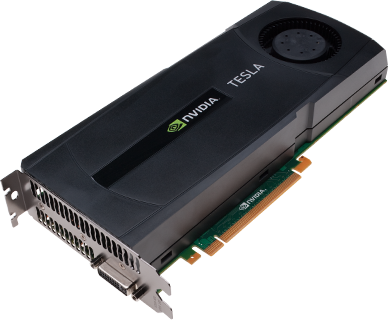
\includegraphics[width=0.2\textwidth]{tesla.png}\quad
        }
        \uncover<1-3>{
            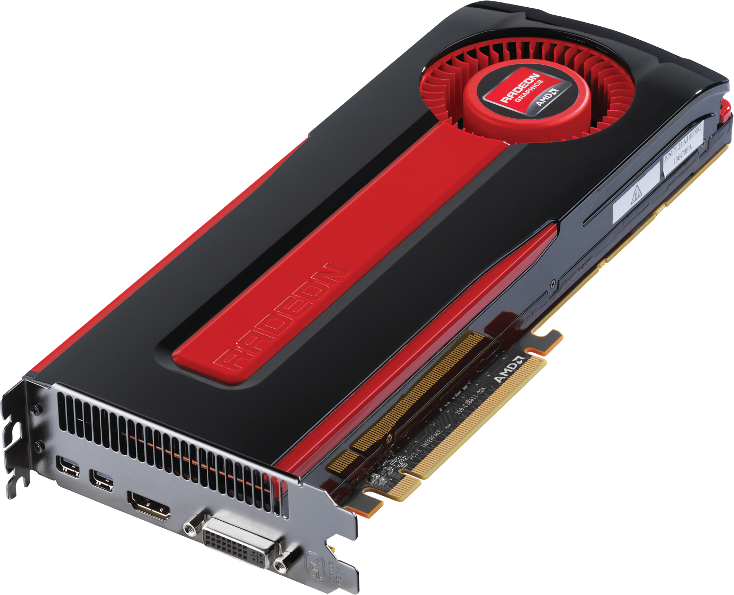
\includegraphics[width=0.2\textwidth]{radeon.png}\quad
        }
        \uncover<1>{
            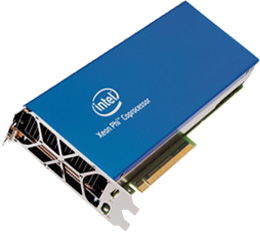
\includegraphics[width=0.16\textwidth]{intel.png}
        }
    \end{figure}
\end{frame}

\note[itemize]{
\item VexCL can transparently work with several compute devices that are
    present on your system.
\item We initialize the VexCL context with a device filter. The device filter
    is a simple functor that acts on cl::Device reference and returns a boolean
    value. Several standard filters are provided and you can write your own
    filters.
\item Let's assume that we have an NVIDIA GPU, an AMD GPU, and an Intel CPU
    installed.
    \begin{enumerate}
        \item The standard 'All' Filter select any device available, so we end
            with three devices in our context.
        \item If we want to select only GPUs, then we can filter the devices by
            type.
        \item It is also possible to combine the device filters with logical
            operators.  Here we select a GPU that is provided by AMD OpenCL
            platform.
        \item And here is an example of a custom filter. Here it selects any
            device that has at least 4GB of memory.
    \end{enumerate}
}

%----------------------------------------------------------------------------
\begin{frame}[fragile]{Exclusive device access}
    \begin{itemize}
        \item \code{vex::Filter::Exclusive()} wraps normal filters to allow
            exclusive access to devices.
        \item Useful in cluster environments.
        \item An alternative to NVIDIA's exclusive compute mode for other
            vendors hardware.
        \item Based on Boost.Interprocess file locks in temp directory.
    \end{itemize}
    \begin{exampleblock}{}
        \begin{lstlisting}
vex::Context ctx( vex::Filter::Exclusive (
    vex::Filter::DoublePrecision && vex::Filter::Env
    ) );
        \end{lstlisting}
    \end{exampleblock}
\end{frame}

\note[itemize]{
\item Often we want to get an exclusive access to our compute devices. This is
    especially true in a clustered environments, where job manager may tell you
    how many devices are available, but it usually doesn't know which exactly.
\item The Exclusive filter wrapper lets you do this. Internally, lock
    files are created for each compute device present in the system.
\item This obviously will only work between VexCL programs that explicitly ask
    for an exclusive access.
}

%----------------------------------------------------------------------------
\begin{frame}[fragile]{Using several contexts}
    \begin{itemize}
        \item Different VexCL objects may be initialized with different VexCL
            contexts.
            \begin{itemize}
                \item Manual work splitting across devices
                \item Doing things in parallel on devices that support it
            \end{itemize}
        \item Operations are submitted to the queues of the vector that is
            being assigned to.
    \end{itemize}
\end{frame}

\note[itemize]{
\item It is possible to initialize different objects with different queue
    lists.  You may want to do this to manually partition the load between
    devices, or to create some non-linear flow in your program.
}

\subsection{Vector arithmetic}

%----------------------------------------------------------------------------
\begin{frame}[fragile]{Vector allocation and arithmetic}
    \begin{exampleblock}{Hello VexCL example}
        \begin{onlyenv}<1|handout:0>
        \begin{lstlisting}[escapechar=!]
vex::Context ctx( !\color{chameleongreen4}{vex::Filter::Name("Tesla")}! );
        \end{lstlisting}
        \end{onlyenv}
        \begin{onlyenv}<2|handout:0>
        \begin{lstlisting}[escapechar=!]
vex::Context ctx( !\color{chameleongreen4}{vex::Filter::Type(CL\_DEVICE\_TYPE\_GPU)}! );
        \end{lstlisting}
        \end{onlyenv}
        \begin{onlyenv}<3>
        \begin{lstlisting}[escapechar=!]
vex::Context ctx( !\color{chameleongreen4}{vex::Filter::DoublePrecision}! );
        \end{lstlisting}
        \end{onlyenv}
        \begin{lstlisting}[firstnumber=last]

vex::vector<float> A(ctx, N); A = 1;
vex::vector<float> B(ctx, N); B = 2;
vex::vector<float> C(ctx, N);

C = A + B;
        \end{lstlisting}
    \end{exampleblock}
    \begin{figure}
        \begin{tikzpicture}
            \draw (0,3.0) rectangle +(8,0.1);
            \draw (0,3.0) grid[step=0.1] +(8,0.1);
            \draw (-0.3,3.1) node{A};

            \draw (0,2.5) rectangle +(8,0.1);
            \draw (0,2.5) grid[step=0.1] +(8,0.1);
            \draw (-0.3,2.6) node{B};

            \draw (0,2.0) rectangle +(8,0.1);
            \draw (0,2.0) grid[step=0.1] +(8,0.1);
            \draw (-0.3,2.1) node[anchor=center]{C};

            \uncover<1-3> {
            \draw (1,0.5) node{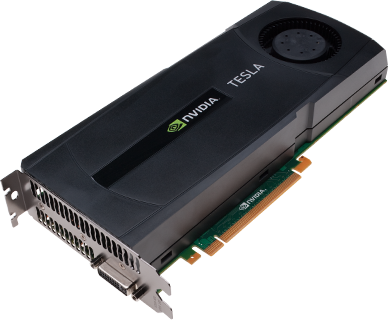
\includegraphics[width=0.2\textwidth]{tesla.png}};
            }

            \uncover<2-3> {
            \draw (4,0.5) node{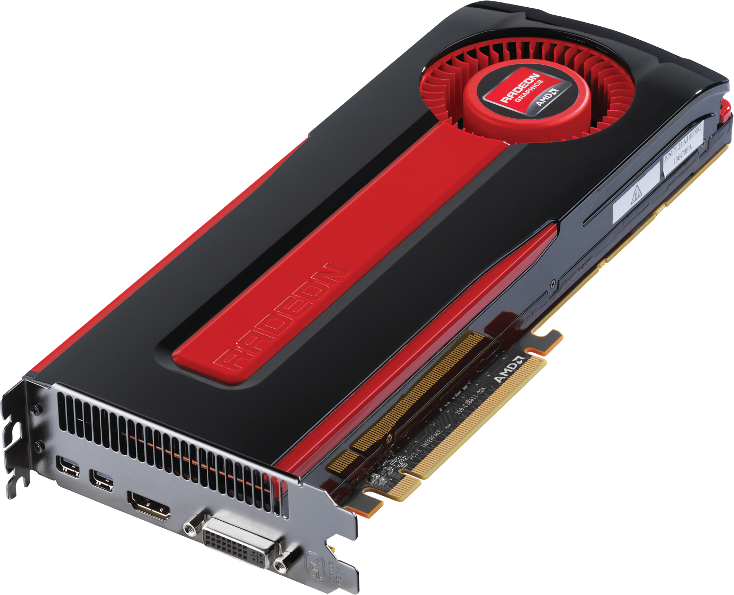
\includegraphics[width=0.2\textwidth]{radeon.png}};
            }

            \uncover<3> {
            \draw (7.5,0.5) node{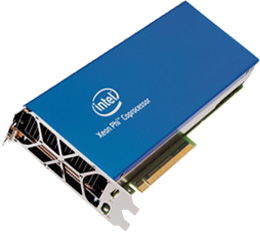
\includegraphics[width=0.16\textwidth]{intel.png}};
            }

            \uncover<1|handout:0> {
            \draw[->,chameleongreen3,style=dashed] (0,3.2) -- (0,1.8)
                .. controls +(east:0.5) and +(north west:0.5) ..
                (1.4,1.5);
            \draw[->,chameleongreen3,style=dashed] (8,3.2) -- (8,1.8)
                .. controls +(west:0.5) and +(north east:0.5) ..
                (1.6,1.5);
            }

            \uncover<2|handout:0> {
            \draw[->,chameleongreen3,style=dashed] (0,3.2) -- (0,1.8)
                .. controls +(east:0.5) and +(north west:0.5) ..
                (1.4,1.5);
            \draw[->,chameleongreen3,style=dashed] (4,3.2) -- (4,1.8)
                .. controls +(west:0.5) and +(north east:0.5) ..
                (1.6,1.5);

            \draw[->,chameleongreen3,style=dashed] (4,3.2) -- (4,1.8)
                .. controls +(east:0.1) and +(north west:0.2) ..
                (4.4,1.5);
            \draw[->,chameleongreen3,style=dashed] (8,3.2) -- (8,1.8)
                .. controls +(west:0.5) and +(north east:0.5) ..
                (4.6,1.5);
            }

            \uncover<3> {
            \draw[->,chameleongreen3,style=dashed] (0,3.2) -- (0,1.8)
                .. controls +(east:0.5) and +(north west:0.5) ..
                (1.4,1.5);
            \draw[->,chameleongreen3,style=dashed] (3.5,3.2) -- (3.5,1.8)
                .. controls +(west:0.5) and +(north east:0.5) ..
                (1.6,1.5);

            \draw[->,chameleongreen3,style=dashed] (3.5,3.2) -- (3.5,1.8)
                .. controls +(east:0.5) and +(north west:0.2) ..
                (4.4,1.5);
            \draw[->,chameleongreen3,style=dashed] (7,3.2) -- (7,1.8)
                .. controls +(west:0.5) and +(north east:0.5) ..
                (4.6,1.5);

            \draw[->,chameleongreen3,style=dashed] (7,3.2) -- (7,1.8) -- (7.4,1.5);
            \draw[->,chameleongreen3,style=dashed] (8,3.2) -- (8,1.8) -- (7.6,1.5);
            }
        \end{tikzpicture}
    \end{figure}
\end{frame}

\note[itemize]{
\item Now that we know how to initialize VexCL context, let's see how device
    vectors are allocated.
\item Here we allocate three vectors, and initialize two of them with
    constant values.
\item Each vector receives a list of queues at initialization.  Since each
    queue corresponds to a specific device, vectors know where to put their
    data to.
    \begin{enumerate}
        \item For example, if we only have the Tesla card in our context, then
            it will hold the complete memory for all of our vectors.
        \item If we use both of the available GPUs, then the vectors will be
            split between the devices. This split is by default proportional to
            the GPU bandwidth and is guaranteed to be consistent for vectors of
            the same size. This consistency allows VexCL to run computations
            independently on all devices in context.
        \item If we add the CPU to the context, it will get smaller share of
            the data and arithmetic operations.
    \end{enumerate}
\item Care must be taken with the use of several devices. VexCL tries to split
    the memory as fair as it can, but it is probable that your program will
    run at the speed of the slowest device.
}

%----------------------------------------------------------------------------
\begin{frame}[fragile]{What may be used in vector expressions?}
    \begin{itemize}
        \item All vectors in expression have to be \emph{compatible}:
            \begin{itemize}
                \item Have same size
                \item Located on same devices
            \end{itemize}
        \item What may be used:
            \begin{itemize}
                \item Scalar values
                \item Arithmetic, bitwise, logical operators
                \item Built-in OpenCL functions
                \item User-defined functions
                \item \ldots
            \end{itemize}
    \end{itemize}
    \begin{exampleblock}{}
        \begin{lstlisting}
std::vector<float> x(n);
std::generate(x.begin(), x.end(), rand);

vex::vector<float> X(ctx, x);
vex::vector<float> Y(ctx, n);
vex::vector<float> Z(ctx, n);

Y = 42;
Z = sqrt(2 * X) + pow(cos(Y), 2.0);
        \end{lstlisting}
    \end{exampleblock}
\end{frame}

\note[itemize]{
\item So, what kind of expressions can you use in VexCL?
\item First, any vectors used in an expression have to be compatible.
\item If this requirement is satisfied, then expressions may combine
    vectors and scalars with almost any binary operators. OpenCL math functions
    and user-defined functions are also available.
}

\subsection{Reductions}

%----------------------------------------------------------------------------
\begin{frame}[fragile]{Reductions}
    \begin{itemize}
        \item Class \code{vex::Reductor<T, kind>} allows to reduce arbitrary
            \emph{vector expression} to a\\ single value of type \code{T}.
        \item Supported reduction kinds: \code{SUM}, \code{MIN}, \code{MAX}
    \end{itemize}
    \begin{exampleblock}{Inner product}
        \begin{lstlisting}
vex::Reductor<double, vex::SUM> sum(ctx);
double s = sum(x * y);
        \end{lstlisting}
    \end{exampleblock}
    \begin{exampleblock}{Number of elements in x between 0 and 1}
        \begin{lstlisting}
vex::Reductor<size_t, vex::SUM> sum(ctx);
size_t n = sum( (x > 0) && (x < 1) );
        \end{lstlisting}
    \end{exampleblock}
    \begin{exampleblock}{Maximum distance from origin}
        \begin{lstlisting}
vex::Reductor<double, vex::MAX> max(ctx);
double d = max( sqrt(x * x + y * y) );
        \end{lstlisting}
    \end{exampleblock}
\end{frame}

\note[itemize]{
\item Reduction is an operation of reducing a vector to a single value.
\item The most frequent types are summation and finding minimum or maximum
    element of a vector.
\item VexCL provides Reductor functor that accepts any valid vector expression
    as a parameter.
\item For example, to compute an inner product of two vectors we compute sum of
    their elementwise product.
\item To find number of elements in vector x that are greater than zero and
    less than one, we compute sum of the corresponding boolean expression.
\item And to find the maximum distance from axis origin for a set of
    two-dimensional points, we compute exactly that: max of their radius.
}

\subsection{User-defined functions}

%----------------------------------------------------------------------------
\begin{frame}[fragile]{User-defined functions}
    \begin{itemize}
        \item Users may define functions to be used in vector expressions:
            \begin{itemize}
                \item Define return type and argument types
                \item Provide function body
            \end{itemize}
    \end{itemize}
    \begin{exampleblock}{Defining a function}
        \begin{lstlisting}[escapechar=!]
VEX_FUNCTION( !\color{chameleongreen4}{between}!, bool(double, double, double),
    "return prm1 <= prm2 && prm2 <= prm3;" );
        \end{lstlisting}
    \end{exampleblock}
    \begin{exampleblock}{Using a function: number of 2D points in first quadrant}
        \begin{lstlisting}[escapechar=!]
size_t points_in_1q( const vex::Reductor<size_t, vex::SUM> &sum,
    const vex::vector<double> &x, const vex::vector<double> &y )
{
    return sum( !\color{chameleongreen4}{between}!(0.0, atan2(y, x), M_PI/2) );
}
        \end{lstlisting}
    \end{exampleblock}
\end{frame}

\note[itemize]{
\item It is possible to define an OpenCL function that may be used with vector
    expressions. You need to provide function body, parameter types, and return
    type.
\item Function body has to be of \code{extern const char} type, to allow its
    use as a template parameter. And it has to be defined at global scope.
\item Inside the body function parameters are always named prm1, prm2, etc.
\item Here we define 'between' function that returns true if its second
    parameter is between its first and third parameters. The UserFunction
    object is stateless, so it may be good idea to define it at global scope
    as well, next to its body.
\item Now we may use the function in expressions. Any vector expression may be
    used as a parameter for a user-defined (or builtin) function.
}

\subsection{Using element indices}


%----------------------------------------------------------------------------
\begin{frame}[fragile]{Using element indices in expressions}
    \begin{itemize}
        \item \code{vex::element_index(size_t offset = 0)} returns index of an
            element inside a vector.
            \begin{itemize}
                \item The numbering starts with \code{offset} and is continuous
                    across devices.
            \end{itemize}
    \end{itemize}
    \begin{exampleblock}{Linear function:}
        \begin{lstlisting}
vex::vector<double> X(ctx, N);
double x0 = 0, dx = 1e-3;
X = x0 + dx * vex::element_index();
        \end{lstlisting}
    \end{exampleblock}
    \begin{exampleblock}{Single period of sine function:}
        \begin{lstlisting}
X = sin(2 * M_PI * vex::element_index() / N);
        \end{lstlisting}
    \end{exampleblock}
\end{frame}

\note[itemize]{
\item \code{element_index} is a function that allows you to use element
    position inside of vector expressions.
\item The function may participate in arbitrary vector expressions.
\item For example, here\ldots
}

\subsection{Random number generation}

%----------------------------------------------------------------------------
\begin{frame}[fragile]{Random number generation}
    \begin{itemize}
        \item VexCL provides implementation\footnote{Contributed by
            \href{https://github.com/neapel}{Pascal Germroth}
            $\langle$\href{mailto:pascal@ensieve.org}{pascal@ensieve.org}$\rangle$}
            of \emph{counter-based} random number generators from
            Random123\footnote{D E Shaw Research,
                \href{http://www.deshawresearch.com/resources\_random123.html}{http://www.deshawresearch.com/resources\_random123.html}}
            suite.
            \begin{itemize}
                \item The generators are \emph{stateless}; mixing functions are
                    applied to element indices.
                \item Implemented families: Threefry and Philox.
            \end{itemize}
    \end{itemize}
    \begin{exampleblock}{Monte Carlo $\pi$:}
        \begin{lstlisting}
vex::Random<double, vex::random::threefry> rnd;          // RandomNormal<> is also available
vex::Reductor<size_t, vex::SUM> sum(ctx);
vex::vector<double> x(ctx, n), y(ctx, n);

x = 2 * rnd(vex::element_index(), std::rand()) - 1;
y = 2 * rnd(vex::element_index(), std::rand()) - 1;

double pi = 4.0 * sum(x * x + y * y < 1) / n;
        \end{lstlisting}
    \end{exampleblock}
\end{frame}

\note[itemize]{
\item Random number generation is a useful feature that is used often in, e.g.,
    molecular dynamics.
\item Random number generators in VexCL are stateless, so they don't require
    additional storage or global memory interactions. Randomness is obtained by
    applying mixing functions to element indices.
}

\subsection{Sparse matrix~-- vector products}

%----------------------------------------------------------------------------
\begin{frame}[fragile]{Sparse matrix~-- vector products \additive}
    \begin{itemize}
        \item Class \code{vex::SpMat<T>} holds representation of a sparse
            matrix on compute devices.
        \item Constructor accepts matrix in common CRS format (row indices,
            columns and values of nonzero entries).
        \item SpMV may only be used in additive expressions.
    \end{itemize}
    \begin{exampleblock}{Construct matrix}
        \begin{lstlisting}
vex::SpMat<double> A(ctx, n, n, row.data(), col.data(), val.data());
        \end{lstlisting}
    \end{exampleblock}

    \begin{exampleblock}{Compute residual value}
        \begin{lstlisting}[firstnumber=last]
// vex::vector<double> u, f, r;
r = f - A * u;
double res = max( fabs(r) );
        \end{lstlisting}
    \end{exampleblock}
\end{frame}

\note[itemize]{
\item Sparse matrix -- vector operation is also provided. A matrix is imported
    from commonly used compressed row storage format.
\item Note that matrix-vector product is not a first-class citizen in vector
    expressions. It uses neighbor values; and neighbors may reside on a
    different compute device. So extra work is needed to exchange data between
    devices. That is why matrix-vector products may only be used in additive
    expressions.
}

\subsection{Stencil convolutions}

%----------------------------------------------------------------------------
\begin{frame}[fragile]{Simple stencil convolutions \additive}
    \begin{figure}
        \begin{tikzpicture}
            \draw[fill,chameleongreen3] (2.6,0.6) rectangle +(0.2,0.2);
            \draw[fill,chameleongreen3] (2.6,0.0) rectangle +(0.2,0.2);

            \draw (0,0) rectangle +(8,0.2);
            \draw (0,0) grid[step=0.2] +(8,0.2);

            \draw (2,0.6) rectangle +(2,0.2);
            \draw (2,0.6) grid[step=0.2] +(2,0.2);

            \draw[chameleongreen3,decorate,decoration={brace,amplitude=5},yshift=2]
                (2,0.85) -- (4.,0.85);
            \draw (3,1.4) node{width};

            \draw (1.9,0.7) node[anchor=east]{$s$};
            \draw (-0.1,0.1) node[anchor=east]{$x$};
            \draw (4.5,0.6) node[anchor=south west]{$y_i=\sum_k s_k x_{i+k}$};
        \end{tikzpicture}
    \end{figure}
    \begin{itemize}
        \item Simple stencil is based on a 1D array, and may be used for:
            \begin{itemize}
                \item Signal filters (e.g. averaging)
                \item Differential operators with constant coefficients
                \item \ldots
            \end{itemize}
    \end{itemize}
    \begin{exampleblock}{Moving average with 5-points window}
        \begin{lstlisting}
std::vector<double> sdata(5, 0.2);
vex::stencil<double> s(ctx, sdata, 2 /* center */);

y = x * s;
        \end{lstlisting}
    \end{exampleblock}
\end{frame}

\note[itemize]{
\item Another commonly used operation is stencil convolution. It may be used to
    filter a one-dimensional signal or to represent a differential operator.
\item A stencil is defined by providing data for its coefficients and
    specifying its center point.
\item To convolve a vector with a stencil you use this simple notation.
\item Stencil convolutions, as well as matrix products, need data from neighbor
    devices; so they may be used only in additive expressions.
}

%----------------------------------------------------------------------------
\begin{frame}[fragile]{User-defined stencil operators \additive}
    \begin{itemize}
        \item Define efficient arbitrary stencil operators:
            \begin{itemize}
                \item Return type
                \item Stencil dimensions (width and center)
                \item Function body
                \item Queue list
            \end{itemize}
    \end{itemize}
    \begin{block}{Example: nonlinear operator}
        \begin{equation*}
            y_i = x_i + \left( x_{i-1} + x_{i+1} \right)^3
        \end{equation*}
    \end{block}
    \begin{exampleblock}{Implementation}
        \begin{lstlisting}
VEX_STENCIL_OPERATOR(custom_op, double, 3/*width*/, 1/*center*/, 
    "double t = X[-1] + X[1];\n"
    "return X[0] + t * t * t;",
    ctx);

y = custom_op(x);
        \end{lstlisting}
    \end{exampleblock}
\end{frame}

\note[itemize]{
\item It is also possible to define a custom stencil operation. This may be
    used, for example, if the stencil operator is nonlinear.
\item For this you specify return type, width of the stencil, its center, and
    function body.
\item In the function body you access values through X array. Its elements are
    indexed relatively to the stencil center.
}

\subsection{Fast Fourier Transform}

%----------------------------------------------------------------------------
\begin{frame}[fragile]{Fast Fourier Transform \additive}
    \begin{itemize}
        \item VexCL provides FFT implementation\footnote{Contributed by 
            \href{https://github.com/neapel}{Pascal Germroth}
            $\langle$\href{mailto:pascal@ensieve.org}{pascal@ensieve.org}$\rangle$}:
            \begin{itemize}
                \item Currently only single-device contexts are supported
                \item Arbitrary vector expressions as input
                \item Multidimensional transforms
                \item Arbitrary sizes
            \end{itemize}
    \end{itemize}
    \begin{exampleblock}{}
        \begin{lstlisting}
vex::FFT<double, cl_double2> fft(ctx, n);
vex::FFT<cl_double2, double> ifft(ctx, n, vex::inverse);

vex::vector<double>     in(ctx, n), back(ctx, n);
vex::vector<cl_double2> out(ctx, n);
// ... initialize 'in' ...

out  = fft(in);
back = ifft(out);
        \end{lstlisting}
    \end{exampleblock}
\end{frame}

\note{
}

\subsection{Multivectors \& multiexpressions}

%----------------------------------------------------------------------------
\begin{frame}[fragile]{Multivectors}
    \begin{itemize}
        \item \code{vex::multivector<T,N>} holds \code{N} instances of equally
            sized \code{vex::vector<T>}
        \item Supports all operations that are defined for
            \code{vex::vector<>}.
        \item Transparently dispatches the operations to the underlying
            components.
        \item \code{vex::multivector::operator(uint k)} returns \code{k}-th
            component.
    \end{itemize}
    \begin{exampleblock}{}
        \begin{lstlisting}
vex::multivector<double, 2> X(ctx, N), Y(ctx, N);
vex::Reductor<double, vex::SUM> sum(ctx);
vex::SpMat<double> A(ctx, ... );
std::array<double, 2> v;

// ...

X = sin(v * Y + 1);             // X(k) = sin(v[k] * Y(k) + 1);
v = sum( between(0, X, Y) );    // v[k] = sum( between( 0, X(k), Y(k) ) );
X = A * Y;                      // X(k) = A * Y(k);
        \end{lstlisting}
    \end{exampleblock}
\end{frame}

\note[itemize]{
\item This is in principle all of the basic VexCL operations.
\item What is left are multivectors and multiexpressions.
}

%----------------------------------------------------------------------------
\begin{frame}[fragile]{Multiexpressions}
    \begin{itemize}
        \item Sometimes an operation cannot be expressed with simple
            multivector arithmetics.
    \end{itemize}
    \begin{block}{Example: rotate 2D vector by an angle}
        \vspace{-1\baselineskip}
        \begin{align*}
            y_0 &= x_0 \cos \alpha - x_1 \sin \alpha, \\
            y_1 &= x_0 \sin \alpha + x_1 \cos \alpha.
        \end{align*}
    \end{block}

    \begin{itemize}
        \item Multiexpression is a tuple of normal vector expressions
        \item Its assignment to a multivector is functionally equivalent to
            component-wise assignment, but results in a single kernel launch.
    \end{itemize}
\end{frame}

\note[itemize]{
\item Sometimes it's not possible to express the required operation with simple
    multivector arithmetics.
\item For example, take two-dimensional point rotation operation, which is
    defined as this couple of expressions. X and Y coordinates are mixed
    here, so we either have to split the operation in two, or use a
    multiexpression.
}

%----------------------------------------------------------------------------
\begin{frame}[fragile]{Multiexpressions}
    \begin{itemize}
        \item Multiexpressions may be used with multivectors:
    \end{itemize}
    \begin{exampleblock}{}
        \begin{lstlisting}
// double alpha;
// vex::multivector<double,2> X, Y;

Y = std::tie( X(0) * cos(alpha) - X(1) * sin(alpha),
              X(0) * sin(alpha) + X(1) * cos(alpha)  );
        \end{lstlisting}
    \end{exampleblock}
    \begin{itemize}
        \item and with tied vectors:
    \end{itemize}
    \begin{exampleblock}{}
        \begin{lstlisting}
// vex::vector<double> alpha;
// vex::vector<double> odlX, oldY, newX, newY;

vex::tie(newX, newY) = std::tie( oldX * cos(alpha) - oldY * sin(alpha),
                                  oldX * sin(alpha) + oldY * cos(alpha)  );
        \end{lstlisting}
    \end{exampleblock}
\end{frame}

\note[itemize]{
\item You can assign a tuple of expressions to a multivector, or to a tuple of
    single vectors.
\item In either case, this will result in single kernel launch that will update
    all parts of the result at once.
\item Also note that in the second example we rotate every point by its own
    angle stored in alpha vector.
}

%----------------------------------------------------------------------------
\begin{frame}[fragile]{Copies between host and device memory}
    \begin{exampleblock}{}
        \begin{lstlisting}
vex::vector<double> X;
std::vector<double> x;
double c_array[100];
        \end{lstlisting}
    \end{exampleblock}
    \begin{exampleblock}{Simple copies}
        \begin{lstlisting}
vex::copy(X, x); // From device to host.
vex::copy(x, X); // From host to device.
        \end{lstlisting}
    \end{exampleblock}
    \begin{exampleblock}{STL-like range copies}
        \begin{lstlisting}
vex::copy(X.begin(), X.end(), x.begin());
vex::copy(X.begin(), X.begin() + 100, x.begin());
vex::copy(c_array, c_array + 100, X.begin());
        \end{lstlisting}
    \end{exampleblock}
    \begin{exampleblock}{Inspect or set single element (\emph{slow})}
        \begin{lstlisting}
assert(x[42] == X[42]);
X[0] = 0;
        \end{lstlisting}
    \end{exampleblock}
\end{frame}

\note[itemize]{
\item Copies between host and device memory may be done with simple copy
    function that copy the complete vector either way,
\item or, if you need to do partial copy, you can use STL-like syntax.
\item Vectors also overload array subscript operator, so you can have direct
    read or write access to any element of a vector. But this should be used
    with caution because it is slow. The intended use for this is a single
    element access or debugging.
\item Data may also be accessed through iterators, so it is possible to use,
    for example, an STL algorithm with device vector as a temporary solution.
}


\section{Performance}

\subsection{Performance}

%----------------------------------------------------------------------------
\begin{frame}[fragile]{Performance}
    \begin{itemize}
        \item Solving ODE (Lorenz attractor ensemble) with Boost.odeint,
            Thrust, and VexCL\footnote{\emph{Programming CUDA and OpenCL: A
            Case Study Using Modern C++ Libraries}.\\
            \hspace{3em}Denis Demidov, Karsten
            Ahnert, Karl Rupp, Peter Gottschling. \href{http://arxiv.org/abs/1212.6326}{arXiv:1212.6326}}
    \end{itemize}
    \begin{description}
        \item[GPU:] NVIDIA Tesla C2070
        \item[CPU:] Intel Core i7 930
    \end{description}

    \begin{figure}
        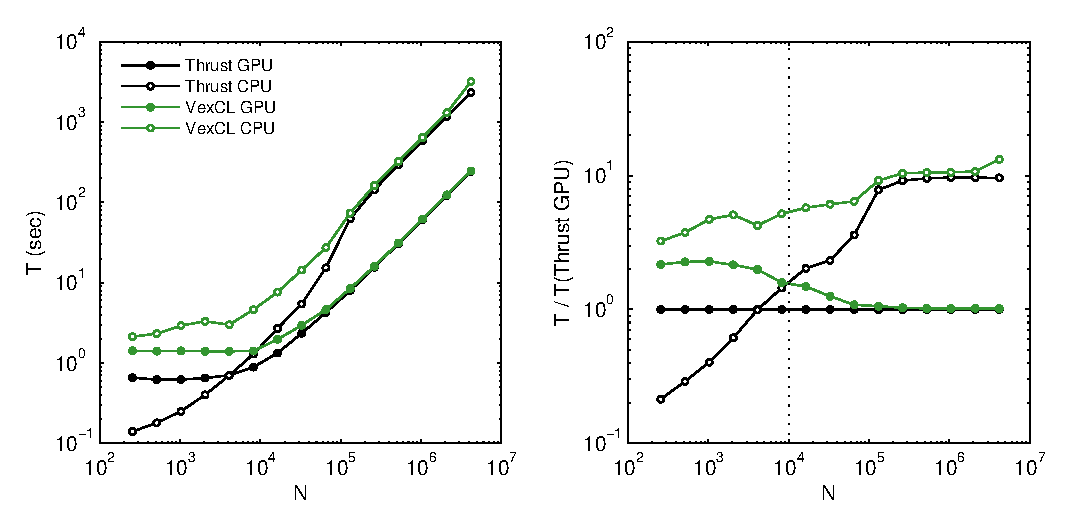
\includegraphics[width=0.75\textwidth]{perfcmp}
    \end{figure}
\end{frame}

\note[itemize]{
\item Here is some data for VexCL performance.
\item We used Boost.Odeint library to solve an ODE with CUDA-based Thrust
    library and with VexCL (the paper referenced here also contains data for
    ViennaCL and CUDA version of MTL). 
\item On the left plot you see absolute running times for problems of different
    sizes. Black lines correspond to
    Thrust based solution on a CPU and GPU, green lines are for VexCL. Filled
    markers are CPU solutions, and empty markers are GPU solutions.
\item Right plot shows running times relative to a Thrust GPU solution.
\item You see that both CUDA and OpenCL have high overhead for small problems,
    so CPU-based Thrust solution is the fastest there.
\item But results for larger problems are much more interesting. Here
    VexCL variant shows performance similar to Thrust's. The solution on a GPU
    is ten times faster than on a CPU for both libraries.
}

%----------------------------------------------------------------------------
\begin{frame}[fragile]{Multigpu scalability}
    \begin{columns}
        \begin{column}{0.45\textwidth}
            \begin{itemize}
                \item \emph{Larger} problems may be solved\\ on the same system.
                \item Large problems may be solved \emph{faster}.
            \end{itemize}
        \end{column}
        \begin{column}{0.5\textwidth}
            \begin{figure}
                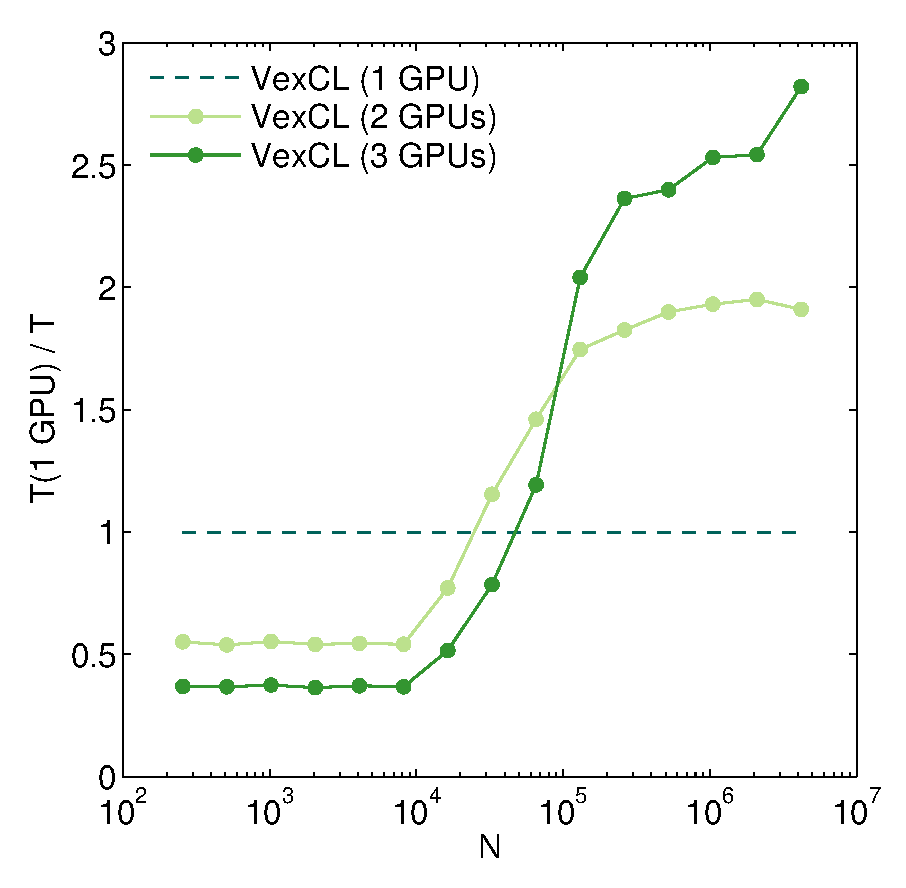
\includegraphics[width=\textwidth]{scaling}
            \end{figure}
        \end{column}
    \end{columns}
\end{frame}

\note[itemize]{
\item Lets see how well VexCL scales with use of multiple GPUs.
\item Here you see acceleration that we get from using several GPUs for the
    same ODE problem.
\item Ideally, we would get double acceleration from two cards, and triple
    acceleration from three cards. And we are getting close to these numbers
    for large problem sizes.
\item Another advantage of multigpu approach is that you can solve larger
    problems on the same system, because memory is split between all of your
    devices.
}

\section{Implementation details}

%----------------------------------------------------------------------------
\begin{frame}{}
    \tableofcontents[currentsection,hideallsubsections]
\end{frame}

\note{ }

\subsection{Expression trees}

%----------------------------------------------------------------------------
\begin{frame}[fragile]{Expression trees}
    \begin{itemize}
        \item VexCL is an \emph{expression template} library.
        \item Boost.Proto is used as an expression template engine.
        \item Each expression in the code results in an expression tree
            evaluated at time of assignment.
            \begin{itemize}
                \item No temporaries are created
                \item Single kernel is generated and executed
            \end{itemize}
    \end{itemize}
    \begin{exampleblock}{Example expression}
        \begin{onlyenv}<1|handout:0>
            \begin{lstlisting}
x = 2 * y - sin(z);
            \end{lstlisting}
        \end{onlyenv}
        \begin{onlyenv}<2>
            \begin{lstlisting}[escapechar=!]
x = !\color{chameleongreen4}{2.0}! * y - sin(z);
            \end{lstlisting}
        \end{onlyenv}
    \end{exampleblock}
    \begin{figure}
        \begin{tikzpicture}
            \draw (0,0) node(minus)[draw,ellipse]{$-$};
            \draw (minus) +(-2, -1) node(times)[draw,ellipse]{$*$};
            \draw (minus) +(2, -1) node(sine)[draw,ellipse]{\code{sin}};
            \uncover<1|handout:0>{
            \draw (times) +(-2,-1) node(const)[draw]{\code{const int&}};
            }
            \uncover<2>{
            \draw (times) +(-2,-1) node(const)[draw,chameleongreen4]{\code{const double&}};
            }
            \draw (times) +(1.5,-1) node(v1)[draw]{\code{const vector<double>&}};
            \draw (sine) +(1.75,-1) node(v2)[draw]{\code{const vector<double>&}};

            \draw (minus) -- (times);
            \draw (minus) -- (sine);
            \draw (times) -- (const);
            \draw (times) -- (v1);
            \draw (sine) -- (v2);
        \end{tikzpicture}
    \end{figure}
\end{frame}

\note[itemize]{
\item Kernel for an expression is generated and compiled only first time the
    expression is encountered. Same overhead exists for manually written OpenCL
    applications.
\item The type of an expression tree encodes types of all its subexpressions,
    so for example this expression would result in a different type and
    different kernel.
\item You should keep this in mind if you want to minimize number of generated
    kernels.
}

\subsection{Kernel generation}

%----------------------------------------------------------------------------
\begin{frame}[fragile]{Kernel generation}
    \begin{columns}
        \begin{column}{0.38\textwidth}
            \begin{exampleblock}{The expression}
                \begin{lstlisting}
x = 2 * y - sin(z);
                \end{lstlisting}
            \end{exampleblock}
        \end{column}
        \begin{column}{0.55\textwidth}
            \emph{Define \code{VEXCL_SHOW_KERNELS} to see the generated code.}
        \end{column}
    \end{columns}
    \begin{exampleblock}{\ldots results in this kernel:}
        \begin{lstlisting}
kernel void minus_multiplies_term_term_sin_term(
    ulong n,
    global double *res,
    int prm_1,
    global double *prm_2,
    global double *prm_3
)
{
    for(size_t idx = get_global_id(0); idx < n; idx += get_global_size(0)) {
        res[idx] = ( ( prm_1 * prm_2[idx] ) - sin( prm_3[idx] ) );
    }
}
        \end{lstlisting}
    \end{exampleblock}
\end{frame}

\note[itemize]{
\item To generate a kernel from an expression VexCL needs to create a parameter
    list for the kernel and the expression string in the kernel body.
\item Expression tree terminals become kernel parameters, and the expression
    string is formed from the information encoded in the expression tree.
\item Here is an example of kernel that is generated from this simple
    expression.
\item If you are curious, you can define \code{VEXCL_SHOW_KERNELS} macro
    before vexcl include pragma. Then sources of every generated kernel will be
    flushed to standard output.
}

\section{Conclusion}

%----------------------------------------------------------------------------
\begin{frame}{Conclusion and Questions}
    \begin{itemize}
        \item VexCL allows to write compact and readable code\\
            without sacrificing performance.
        \item Multiple compute devices are employed transparently.
        \item Supported compilers (don't forget to enable C++11 features):
            \begin{itemize}
                \item GCC v4.6
                \item Clang v3.1
                \item MS Visual C++ 2010
            \end{itemize}
    \end{itemize}

    \begin{columns}
        \begin{column}{0.5\textwidth}
            \begin{itemize}
                \item \href{https://github.com/ddemidov/vexcl}
                    {https://github.com/ddemidov/vexcl}
            \end{itemize}
        \end{column}
        \begin{column}{0.25\textwidth}
            \begin{figure}
                
\includegraphics[width=0.6\textwidth]{octocat}
            \end{figure}
        \end{column}
        \begin{column}{0.1\textwidth}
        \end{column}
    \end{columns}
\end{frame}

\note{ }


\end{document}


% vim: et
